La conocida sucesión de Fibonacci es aquella sucesión que comienza con los términos 0 y 1, y continua obteniendo cada término sumando sus dos anteriores. Mas formalmente: 

\begin{figure}[h]
	\centering
	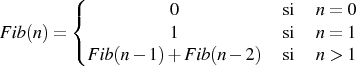
\includegraphics[width=0.5\linewidth]{img/generalizacion-fibonacci-1}
	\label{fig:generalizacion-fibonacci-1}
\end{figure}

Esta sucesión o alguna se sus variantes esta presente en varios problemas de concursos por lo cual es vital que un concursante sepa cuales son las maneras de calcular cualquier elemento de sucesión conociendo el orden de este dentro de la sucesión, así como las propiedades que presenta la sucesión.